\documentclass{beamer}
\usepackage{color} %For Comments
\usepackage{beamerthemeshadow}
\mode<presentation>
{
\usetheme{Montpellier}
\usecolortheme{dolphin}
%%% set style for ovelays: lists (and other text) appearing one item at a time
%%% This will create a dimmed preview of next item:
%\setbeamercovered{transparent}
%%% This will hide it entirely:
\setbeamercovered{invisible}
}

%% Elena's favorite green (thanks, Fernando!)
\definecolor{ForestGreen}{RGB}{34,139,34}
\definecolor{BlueViolet}{RGB}{138,43,226}
\definecolor{Coquelicot}{RGB}{255, 56, 0}
\definecolor{Teal}{RGB}{2,132,130}
% Uncomment this if you want to show work-in-progress comments
\newcommand{\comment}[1]{{\bf \tt  {#1}}}
% Uncomment this if you don't want to show comments
%\newcommand{\comment}[1]{}
\newcommand{\emcomment}[1]{\textcolor{ForestGreen}{\comment{Elena: {#1}}}}
\newcommand{\todo}[1]{\textcolor{blue}{\comment{To Do: {#1}}}}
\newcommand{\hfcomment}[1]{\textcolor{Teal}{\comment{Henry: {#1}}}}
\newcommand{\thcomment}[1]{\textcolor{Coquelicot}{\comment{Thomas: {#1}}}}
\newcommand{\R}[1]{\textcolor{blue}{\bf {#1}}}
\newcommand{\Cl}[1]{\textcolor{ForestGreen}{\bf {#1}}}
\newcommand{\NoJava}[1]{\textcolor{purple}{\bf {#1}}}
%%%%%%%%%%%%%%%%%%%%%%%%%%%%%%%%%%%%%%%%%%

\begin{document}
\title{Usability of beginner-oriented Clojure error messages}
\author{Henry Fellows, Thomas Hagen, Sean Stockholm, 
and Elena Machkasova}
\institute[UMM] % (optional, but mostly needed)
{
 % \inst{1}%
  University of Minnesota, Morris
}
\date{5th International Workshop on Trends in Functional Programming in Education, \\
College Park, MD, June 7, 2016}

\begin{frame}
\titlepage
\end{frame}
%frame

\begin{frame}
\frametitle{Table of contents}
\tableofcontents  
\end{frame}

\section{Overview}

\begin{frame}
\frametitle{Clojure and goals of our project }
Clojure:
\begin{itemize}
\item A Lisp, runs on the JVM
\item Data immutable; state is handled explicitly 
\item Support for concurrency 
\item Rich collection of data structures (lists, vectors, hashmaps, sets,...)
\item Developed by Rich Hickey, released in 2007
\item Has a large community of users and developers 
\end{itemize}

A project at University of Minnesota, Morris (UMM) to make it possible to use Clojure as the first language for teaching beginner students. 
\end{frame}

\begin{frame}
\frametitle{UMM course structure}
UMM current course structure:
\begin{itemize}
\item Introductory: Racket or Python 
\item Second programming course: Data Structures in Java
\item Upper level classes use a variety of languages:  Javascript (web development), C, Ruby (operating systems),  R, Clojure (data processing). 
\end{itemize} 
Seeing a functional language first is helpful (functional abstraction, higher-order functions). 

%Students have no problem picking up new languages. 
\end{frame}

\begin{frame}
\frametitle{Clojure in introductory class}
Clojure is a promising language for an introductory class:
\begin{itemize}
\item Functional language
\item Provides a large set of data structures (hashmaps, sets)
 \item Has a large community of developers and users: libraries, participation in open source projects, parallel data processing,  etc. 
\end{itemize} 
\end{frame}

\begin{frame}[fragile]
\frametitle{Challenges for using Clojure in introductory class}
Challenges:
\begin{itemize}
\item Beginner-friendly IDEs are still under development
\item Syntax is very flexible, so errors are detected late. Example: \\ 
{(first '())} returns {\tt nil}, may cause null pointer exception later.  
\item Errors are Java exceptions, are phrased in terms of Java types:
\begin{verbatim}
>(+ "hi")
java.lang.ClassCastException: 
Cannot cast java.lang.String to java.lang.Number
\end{verbatim}
\end{itemize}
Our work: providing beginner-friendly error messages for Clojure. 
\end{frame}

\begin{frame}
\frametitle{ Our project}
To develop materials and setup that would make it possible to use Clojure in an introductory class. 
\begin{itemize}
\item Modifying error messages
\item Evaluating how well new error messages work: usability study comparing our error messages to standard ones and to Racket
\item Future work: integrate our messages into an IDE 
\item Other work: graphical library that abstracts over state and objects; developing lecture notes 
\end{itemize}
\end{frame}

\begin{frame}
\frametitle{ Our project}
To develop materials and setup that would make it possible to use Clojure in an introductory class. 
\begin{itemize}
\item {\bf Modifying error messages}
\item {\bf Evaluating how well new error messages work: usability study comparing our error messages to standard ones and to Racket}
\item Future work: integrate our messages into an IDE
\item Other work: graphical library that abstracts over state and objects; developing lecture notes 
\end{itemize}
\end{frame}

\section{Modifying error messages}

\begin{frame}[fragile]
\frametitle{ Clojure error messages: example}
Code: {\tt (+ 1 "hi")}

Standard Clojure error:
\begin{verbatim}
java.lang.ClassCastException: 
	java.lang.String cannot be cast to java.lang.Number
	clojure.lang.Numbers/add (Numbers.java line 128)
	clojure.lang.Numbers/add (Numbers.java line 3640)
	intro.test/eval8691 (test_standard.clj line 8)
	clojure.lang.Compiler/eval (Compiler.java line 6792)
	clojure.lang.Compiler/load (Compiler.java line 7237)
	clojure.lang.Compiler/loadFile (Compiler.java line 7175)
	clojure.lang.RT$3/invoke (RT.java line 319)
	intro.core/-main (core.clj line 19)
	....>15  more stack trace lines....
\end{verbatim}
\end{frame}

\begin{frame}[fragile]
\frametitle{ Clojure error messages: example}
Our error message for the same code  {\tt (+ 1 "hi")}:
\begin{verbatim}
Error: In function +, the second argument "hi" must be 
a number but is a string.
Found in file 
C:\Users\E\Desktop\clojure-intro-class\src\intro\test.clj 
on, or before, line 8.
	corefns.corefns/+ (corefns.clj line 269)
	intro.test/eval8691 (test.clj line 11)
	intro.core/-main (core.clj line 20)
\end{verbatim}
\end{frame}

\begin{frame}
\frametitle{Our approach}
\begin{itemize}
\item Can't just surround the program with try/catch: compilation errors and lazy sequences evaluation errors escape to REPL
\item For now: load user's code via {\tt eval}, catch errors
\item Two approaches:
	\begin{itemize}
	\item Overwrite core functions to add pre-conditions: {\tt +} takes numbers, {\tt first} takes a sequence, etc. Can print 		arguments that fail preconditions
	\item Catch error messages and transform them using regular expressions
	\end{itemize}
\item Filter stack trace
\end{itemize}
Anecdotal evidence: this works well, catches most cases. 
\end{frame}


\section{Usability study}

\begin{frame}
\frametitle{Usability study}
Usability study questions:
\begin{enumerate}
\item How do our error messages compare to standard Clojure messages?
\item How do they compare to Racket? %(Many UMM students are familiar with Racket)
\item What works well, what needs improvement? 
\end{enumerate}
Ideas for the study:

Marceau et al 2011 {\it Measuring effectiveness  of Error Messages Designed for Novice Programmers}, 

Mayer et al 2012 {\it  An empirical study of the influence of static
type systems on the usability of undocumented software}. 

%\emcomment{add a reference to the Racket paper and the static/dynamic typing paper}

{\bf Study is in progress, we are presenting preliminary results.}
\end{frame}

\begin{frame}
\frametitle{Usability study}
%Usability study:
\begin{itemize}
\item 16 program fragments with errors, each has a Racket and a Clojure version 
\item Divided into 4 levels by difficulty
\item Each participant gets 2 Racket, 2 Clojure questions at each level
\item Randomly assigned standard/modified Clojure error messages
\item Overview of Racket, 8 Racket questions 
\item Overview of Clojure, 8 Clojure questions
\item Screen capture while solving questions (21 minutes each set)
\item A short interview at the end
\end{itemize}
\end{frame}

\begin{frame}
\frametitle{ Clojure and Racket: common elements}
For the study we picked a common subset of Racket and Clojure familiar to students:
\begin{itemize}
\item Numbers, booleans, lists
\item Functions and variables definitions
\item {\tt if, cond}
\item Structures (Racket), hashmaps (Clojure)
\item Recursion
\item Higher-order functions: {\tt map, filter, reduce/fold}
\item Anonymous functions
\end{itemize}
\end{frame}

\begin{frame}[fragile]
\frametitle{ Clojure and Racket:  differences}
\begin{itemize}
\item Syntax differences in function definitions:
\begin{verbatim}
(define (f x) (+ x 2)) ; Racket

(defn f [x] (+ x 2)) ; Clojure
\end{verbatim}
\item Structures in Racket vs hashmaps in Clojure:
\begin{verbatim}
;; Structure in Racket
(define-struct point (x y))
(define point1 (make-point 5 7))
(point-x point1)

;; Clojure hashmaps
(def point1 {:x 5, :y 7})
 (:x point1)
\end{verbatim}
\item {\tt fold} vs {\tt reduce}, {\tt nil} handling, etc. 
\end{itemize}
%\emcomment{Features we are not using in  Clojure}
\end{frame}

\begin{frame}
\frametitle{ Clojure features not included}
Not included in the study:
\begin{itemize}
\item Strings 
\item Vectors, {\tt conj, into}
\item loop/recur
\item Function literals, such as {\tt \#(\% + 2)} 
\item Many higher-order functions
\item Automated testing (in either language)
\end{itemize}
Some code in our examples isn't idiomatic. 
\end{frame}

\begin{frame}
\frametitle{Racket testing environment}
\begin{figure}
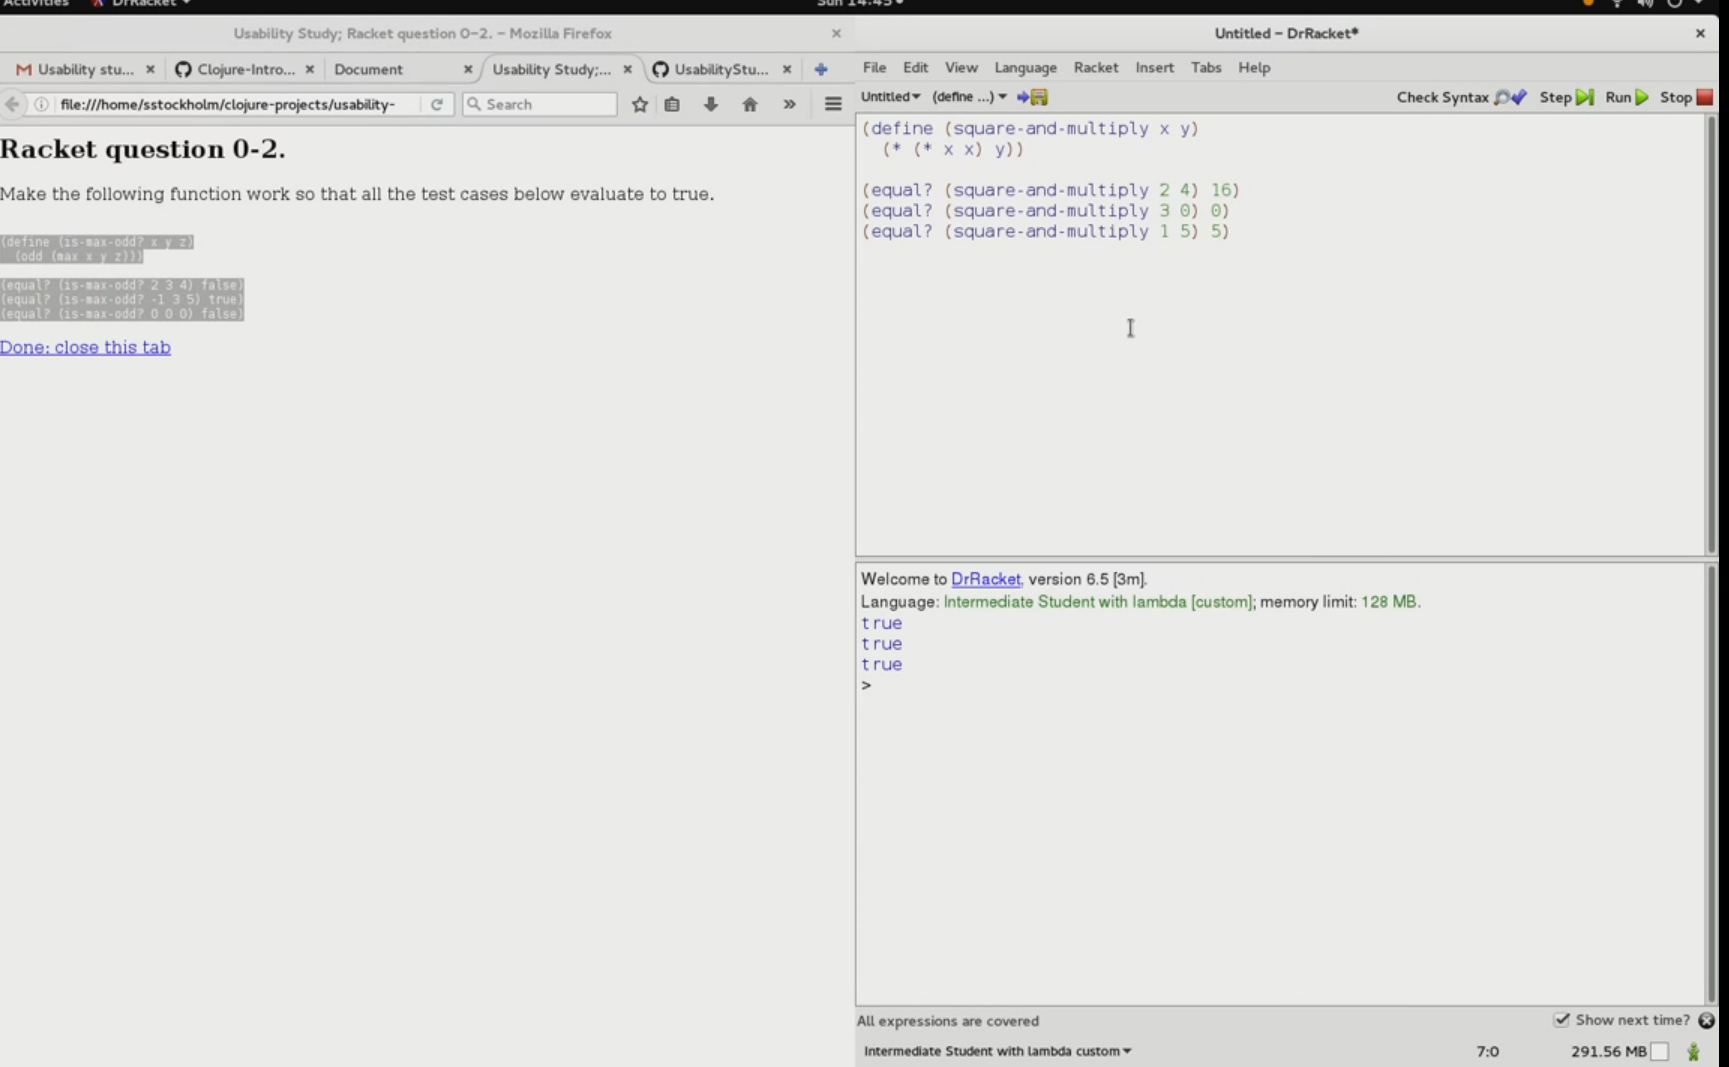
\includegraphics[height=0.75\textheight]{RacketEnvironment.png}
\caption{Racket testing environment: DrRacket,  intermediate w/lambda}
\end{figure}
\end{frame}


\begin{frame}
\frametitle{Clojure testing environment}
\begin{figure}
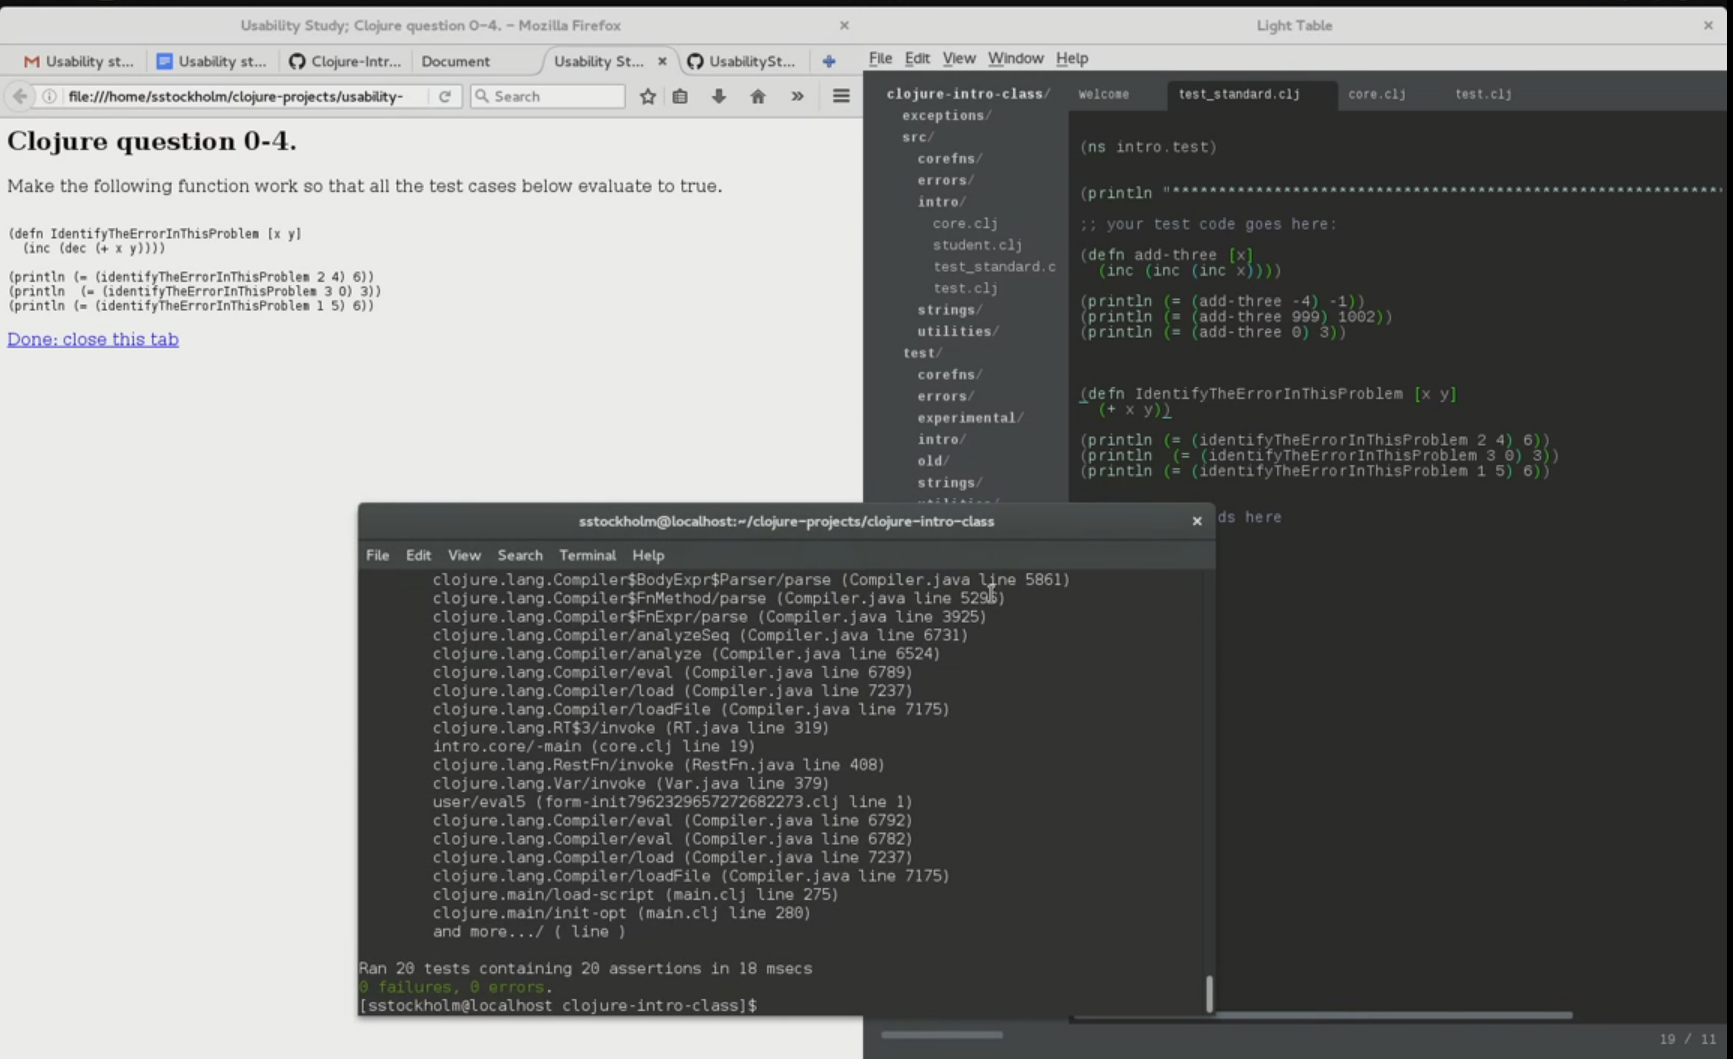
\includegraphics[height=0.75\textheight]{ClojureEnvironment.png}
\caption{Clojure testing environment: LightTable IDE, leiningen project }
\end{figure}
\end{frame}

\begin{frame}[fragile]
\frametitle{Study questions (easy)}
{\it Make the following function work so that all the test cases below evaluate to true. }
\begin{verbatim}
(define (square-and-multiply x y) ;;; Racket
  (* (* X X) y))

(equal? (square-and-multiply 2 4) 16)
(equal? (square-and-multiply 3 0) 0)
(equal? (square-and-multiply 1 5) 5)
\end{verbatim}

\begin{verbatim}
(defn square-and-multiply [x y] ;;; Clojure
  (* (* X X) y))
\end{verbatim}
\end{frame}

\begin{frame}[fragile]
\frametitle{Study questions (easy)}
%%{\it Make the following function work so that all the test cases below evaluate to true. }
\begin{verbatim}
(define (square-and-multiply x y) ;;; Racket
  (* (* X X) y))
\end{verbatim}
Racket error: {\tt X: this variable is not defined} 

\begin{verbatim}
(defn square-and-multiply [x y] ;;; Clojure
  (* (* X X) y))
\end{verbatim}

Clojure standard: {\tt java.lang.RuntimeException: Unable to resolve symbol: X in this context}


\vspace*{.2in}

Our Clojure: {\tt Syntax error: Name X is undefined}

\end{frame}

\begin{frame}[fragile]
\frametitle{Study questions (harder)}
\begin{verbatim}
(define (large-evens numbers bound)
  (filter (lambda (x) (>= x bound))
          (map even? numbers)))

(equal? (large-evens '(22 23 5 30 27 4) 5) '(22 30))
(equal? (large-evens '(22 23 5 30 27 4) 3) '(22 30 4))
(equal? (large-evens '(22 23 5 30 27 4) 40) '())
\end{verbatim}
\begin{verbatim}
(defn large-evens [numbers bound]
  (filter (fn [x] (>= x bound))
          (map even? numbers)))
\end{verbatim}
\end{frame}

\begin{frame}[fragile]
\frametitle{Study questions (harder)}
Racket error: {\tt >=: expects a real as 1st argument, given true}

\vspace*{.2in}

Standard Clojure: {\tt java.lang.ClassCastException: java.lang.Boolean cannot be cast to java.lang.Number}

\vspace*{.2in}

Our Clojure: {\tt Error: In function >=, the first argument {\bf true}  must be a number but is a boolean.}
\end{frame}

\section{Results}

\begin{frame}
\frametitle{Study participants overview}
\begin{itemize}
\item Have had the class that used Racket
\item Are not very familiar with Clojure 
\item Participants invited via department mailing list and old class lists (some additionally personally invited)
\item A study takes 1-1.5 hours, compensated for their time (to increase diversity)
\item So far: 11 participants: 10 male, 1 female; range from first year to seniors; CS majors and non-majors.  
%\item Racket-based class: Fall 2015: 4, Fall 2014: 5, Earlier: 2. 
%\item Good at Racket: 2, were good at Racket, but forgot: 8, find Racket challenging: 1.
%\item Somewhat familiar with Clojure: 6, not familiar: 5.  
\end{itemize}
\end{frame}

\begin{frame}
\frametitle{Results}
%\emcomment{Results: questions solved and times}
{\bf Standard error messages} 
\vspace{0.1in}

\begin{tabular}{c | c| c| c | c }
\hline
{\bf ID} & {\bf Racket  \#} & {\bf Racket time} & {\bf Clojure  \#} & {\bf Clojure time} \\
\hline 
14 &  8 & 12min 20sec &  6  &  21min \\
17 &  8 & 19min 58 sec &  7 &  21min \\
20* &  6 & 21min &  4 &  21min \\
23 &  7 & 21min &  6  &  21min \\
26 &  8 & 14min 21sec &  6 &  21min \\
\hline
\end{tabular}

*Participant 20 by mistake had two questions being the same in Racket and Clojure. 
\end{frame}

\begin{frame}
\frametitle{Results}
%\emcomment{Results: questions solved and times}
{\bf Modified (our) error messages}
\vspace{0.1in}

\begin{tabular}{c | c| c| c | c }
\hline
{\bf ID} & {\bf Racket  \#} & {\bf Racket time} & {\bf Clojure  \#} & {\bf Clojure time} \\
\hline 
2 & 7  & 20min 56sec & 8 & 16min 22sec  \\
6 &  8  & 14min 25sec &  4  &  21min \\
13 &  8 & 7min 53sec &  7 &  21min \\
16 &  8  & 14min 41sec &  8  &  15min 53sec \\
25 &  8  & 16min 46sec &  8  &  13min 9sec \\
29 &  4  & 21min &  2  &  21min \\
\hline
\end{tabular}
\end{frame}

\begin{frame}
\frametitle{Results}
%\emcomment{Results: questions solved and times}
{\bf Standard error messages: \Cl{background in Clojure}, \R{recent Racket}}
\vspace{0.1in}

\begin{tabular}{c | c| c| c | c }
\hline
{\bf ID} & {\bf Racket  \#} & {\bf Racket time} & {\bf Clojure \#} & {\bf Clojure time} \\
\hline 
14 &  8 & 12min 20sec &  \Cl{6}  &  \Cl{21min} \\
17 &  8 & 19min 58 sec &  7 &  21min \\
20* &  6 & 21min &  4 &  21min \\
23 &  7 & 21min &  6  &  21min \\
26 &  \R{8} & \R{14min 21sec} &  \Cl{6} &  \Cl{21min} \\
\hline
\end{tabular}
Even those who claim to know Clojure took the entire time and didn't solve all the questions. 

%*Participant 20 by mistake had two questions being the same in Racket and Clojure. 
\end{frame}

\begin{frame}
\frametitle{Results}
%\emcomment{Results: questions solved and times}
{\bf Modified (our) error messages:  \Cl{background in Clojure}, \R{recent Racket}, \NoJava{not familiar with Java}}
\vspace{0.1in}

\begin{tabular}{c | c| c| c | c }
\hline
{\bf ID} & {\bf Racket  \#} & {\bf Racket time} & {\bf Clojure  \#} & {\bf Clojure time} \\
\hline 
2 & 7  & 21min 56sec &  \Cl{8} & \Cl{16min 22sec} \\
6 &  8  & 14min 25sec &  4  &  21min \\
13 &  \R{8}  & \R{7min 53sec} &  \Cl{7}  &  \Cl{21min} \\
16 &  8  & 14min 41sec &  \Cl{8}  &  \Cl{15min 53sec} \\
25 &  8  & 16min 46sec &  \Cl{8}  &  \Cl{13min 9sec} \\
29 &  4  & 21min &  \NoJava{2}  & \NoJava{21min} \\
\hline
\end{tabular}
For those somewhat familiar with Clojure results are closer to Racket. 
\end{frame}


\begin{frame}
\frametitle{Other parameters measured}
We also measured:
\begin{itemize}
\item Amount of time on track. So far there doesn't seem to be a significant difference (most participants are on track most or all of the time). 
\item %However, even when a participant is looking for the right thing, 
Standard Clojure makes a specific place and cause of the error difficult to find. Example: a subtly misspelled function name leads to "name ... undefined" error. Participants  look for proper syntax for function definition: reasonable interpretation of the message. 
\item Number of runs per question attempted. Ranges between 1.25 and 4. No clear correlations at this point. 
\end{itemize}
\end{frame}

%\begin{frame}
%\frametitle{Results:interview questions}
%\emcomment{Interview questions and feedback}
%\end{frame}

\section{Conclusions and future work}

\frametitle{Conclusions}

\begin{frame}
Preliminary conclusions:
\begin{itemize}
\item Standard Clojure messages make it difficult to solve all questions. Our modified messages make results closer to Racket, especially for 
those somewhat familiar with Clojure
\item The stack trace in standard Clojure is overwhelming, makes it hard to find errors 
\end{itemize}
Hypotheses with not enough data (but some anecdotal evidence):
\begin{itemize}
\item For easier questions all error messages are sufficient
\item Differences show up more in harder questions 
\item Java background helps in understanding standard error messages
\end{itemize}
\end{frame}

\begin{frame}
\frametitle{Thoughts on the usability study}
\begin{itemize}
\item Need to make an effort to get a diverse population. Would like to get more non-CS majors with no Java background
\item Screen capture helps in tracking participants' thought process
\item Putting together a good set of questions is challenging
\item Comparing to Racket provides a useful, but not perfect, way of estimating participants' level 
\item Question-by-question comparison between different languages would be interesting
\end{itemize}
\end{frame}

\begin{frame}
\frametitle{Future work}
Work on the study:
\begin{itemize}
\item Recruit a more diverse (by background) participants' group
\item Analyze specifics of actions, question-by-question
\end{itemize}
General directions:
\begin{itemize}
\item Work on improving error messages based on the study
\item Work on incorporating error messages into an IDE (collaboration with IDE developers)
\item Wrap up development of course material, teach a class to a small group of students 
\end{itemize}
\end{frame}

\begin{frame}
\frametitle{Acknowledgments}
Thanks to...
	\begin{itemize}
	\item HHMI, UMN UROP, LSAMP 
	\item UMM Research students: Myeongjae (Tony) Song, Richard Stangl, and Shamund Gordon 
        \item Coginitect, Inc providing funding for participants' compensation 
	\item Study participants 
	\end{itemize}
	{\centering
	\noindent
	Questions? \par
	}
\end{frame}
\end{document}
